\subsection{Functional Requirements}

Các yêu cầu chức năng được tổ chức theo từng module. Những chức năng đã triển khai thành công được đánh dấu \checkmark, các chức năng chưa hỗ trợ để trống.

\begin{itemize}

\item \textbf{Scheduling Module}

\begin{longtable}{|p{10cm}|c|}
\caption{Scheduling Module}
\hline
\textbf{Chức năng} & \textbf{Trạng thái} \\
\hline
Xem lịch làm việc cá nhân & \checkmark \\ \hline
Xem chi tiết ca làm việc (giờ bắt đầu, kết thúc, vị trí) & \checkmark \\ \hline
Xem danh sách ca mở và đăng ký ca mở & \checkmark \\ \hline
Gửi đơn nghỉ phép (bao gồm nghỉ khẩn cấp, có đề xuất thay thế) & \checkmark \\ \hline
Quản lý trạng thái và lịch sử đơn nghỉ phép & \checkmark \\ \hline
Hủy đơn nghỉ phép chưa được duyệt & \checkmark \\ \hline
Theo dõi số dư ngày nghỉ phép còn lại & \checkmark \\ \hline
Xem dashboard tổng quan lịch làm việc & \checkmark \\ \hline
Thêm, sửa, xóa ca làm việc & \checkmark \\ \hline
Sao chép ca làm sang ngày/tuần khác & \checkmark \\ \hline
Hệ thống gợi ý phân công ca phù hợp & \checkmark \\ \hline
Phê duyệt hoặc từ chối đơn nghỉ phép & \checkmark \\ \hline
Tạo đơn nghỉ thay nhân viên và điều chỉnh số dư nghỉ & \checkmark \\ \hline
Xuất bản lịch làm việc chính thức &  \\ 
\hline
\end{longtable}

\item \textbf{Menu Module}

\begin{longtable}{|p{10cm}|c|}
\caption{Menu Module}
\hline
\textbf{Chức năng} & \textbf{Trạng thái} \\
\hline
Quản lý sản phẩm (tạo, sửa, xóa, cập nhật giá, hình ảnh, trạng thái) & \checkmark \\ \hline
Quản lý danh mục sản phẩm (tạo, sửa, xóa, phân cấp cha-con, đếm sản phẩm) & \checkmark \\ \hline
Quản lý combo món ăn (tạo combo, thêm món, thiết lập giá combo) & \checkmark \\ \hline
Quản lý thuộc tính sản phẩm (size, màu sắc, biến thể) & \checkmark \\ \hline
Quản lý hình ảnh sản phẩm & \checkmark \\
\hline
\end{longtable}

\item \textbf{POS – Ăn tại chỗ}

\begin{longtable}{|p{10cm}|c|}
\caption{POS – Ăn tại chỗ}
\hline
\textbf{Chức năng} & \textbf{Trạng thái} \\
\hline
Xem trạng thái bàn (trống, đã chiếm, đã đặt trước) & \checkmark \\ \hline
Bắt đầu và tiếp tục đơn hàng theo bàn & \checkmark \\ \hline
Thêm món và biến thể vào đơn & \checkmark \\ \hline
Hủy món hoặc đơn hàng (có lý do và duyệt quản lý) & \checkmark \\ \hline
Thanh toán (tiền mặt, thẻ, ví điện tử, tip) & \checkmark \\ \hline
Hoàn tất đơn hàng và giải phóng bàn & \checkmark \\ \hline
Khởi tạo phiên POS (ghi nhận số dư đầu ca, nhân viên mở ca) &  \\ \hline
Di chuyển hoặc gộp đơn hàng giữa các bàn &  \\ \hline
Tạo hóa đơn tạm tính &  \\ \hline
Chia hóa đơn (theo món hoặc theo người) &  \\ 
\hline
\end{longtable}

\item \textbf{POS – Mang về}

\begin{longtable}{|p{10cm}|c|}
\caption{POS – Mang về}
\hline
\textbf{Chức năng} & \textbf{Trạng thái} \\
\hline
Chuyển POS sang chế độ mang về & \checkmark \\ \hline
Tạo đơn hàng mang về (không gắn bàn) & \checkmark \\ \hline
Liên kết khách hàng (tên, số điện thoại) & \checkmark \\ \hline
Thêm món và biến thể vào đơn mang về & \checkmark \\ \hline
Thêm ghi chú đặc biệt cho đơn mang về & \checkmark \\ \hline
Định tuyến món mang về đến bếp/KDS & \checkmark \\ \hline
Thanh toán mang về (tiền mặt, thẻ, ví điện tử) & \checkmark \\
\hline
\end{longtable}

\item \textbf{Đặt bàn \& Pre-order}

\begin{longtable}{|p{10cm}|c|}
\caption{Đặt bàn \& Pre-order}
\hline
\textbf{Chức năng} & \textbf{Trạng thái} \\
\hline
Hiển thị khung giờ và bàn trống & \checkmark \\ \hline
Hiển thị sơ đồ bàn và chọn bàn trống & \checkmark \\ \hline
Xem danh sách món từ thực đơn & \checkmark \\ \hline
Thêm món và biến thể vào giỏ đặt trước & \checkmark \\ \hline
Tính tiền cọc (theo \% cấu hình) & \checkmark \\ \hline
Tích hợp cổng thanh toán và lưu giao dịch & \checkmark \\ \hline
Hoàn tất đặt chỗ, gửi email/SMS, cập nhật trạng thái bàn & \checkmark \\ \hline
Trừ tiền cọc từ hóa đơn POS & \checkmark \\ \hline
Thêm món đặt trước vào đơn POS & \checkmark \\ \hline
Quản lý danh sách đặt chỗ (online/offline) & \checkmark \\ \hline
Xem chi tiết đặt chỗ (khách, món, thanh toán) & \checkmark \\ \hline
Cập nhật trạng thái đặt chỗ (Xác nhận, Đã đến, Hủy) & \checkmark \\ \hline
Xem lịch sử đặt chỗ của khách & \checkmark \\ \hline
Nhân viên tạo/chỉnh sửa đặt chỗ qua điện thoại &  \\ \hline
Báo cáo món đặt trước cho ca sắp tới &  \\ 
\hline
\end{longtable}

\item \textbf{Kitchen/KDS}

\begin{longtable}{|p{10cm}|c|}
\caption{Kitchen/KDS}
\hline
\textbf{Chức năng} & \textbf{Trạng thái} \\
\hline
Gửi món từ POS đến bếp/KDS & \checkmark \\ \hline
Hiển thị danh sách đơn và chi tiết món trên KDS & \checkmark \\ \hline
Đánh dấu món/đơn là đang làm hoặc hoàn tất & \checkmark \\ \hline
Hiển thị thông tin món (tên, số lượng, biến thể, ghi chú) & \checkmark \\ \hline
Sắp xếp hoặc ưu tiên đơn hàng trên KDS & \checkmark \\ \hline
Đồng bộ trạng thái món từ KDS về POS & \checkmark \\
\hline
\end{longtable}

\item \textbf{POS – Giao hàng}

\begin{longtable}{|p{10cm}|c|}
\caption{POS – Giao hàng}
\hline
\textbf{Chức năng} & \textbf{Trạng thái} \\
\hline
Tạo đơn giao hàng (thông tin khách, địa chỉ) & \checkmark \\ \hline
Liên kết đơn với khách (tên, số điện thoại, địa chỉ) & \checkmark \\ \hline
Thêm món và biến thể vào đơn giao hàng & \checkmark \\ \hline
Thêm ghi chú đặc biệt cho đơn giao hàng & \checkmark \\ \hline
Định tuyến món giao hàng đến bếp/KDS & \checkmark \\ \hline
Chuyển POS sang chế độ giao hàng &  \\ \hline
Tích hợp Shipday (gửi đơn, địa chỉ, thông tin khách) &  \\ \hline
Webhook nhận trạng thái giao hàng (Đã giao, Thất bại) &  \\ \hline
Ghi nhận thanh toán khi giao hàng (COD) &  \\ 
\hline
\end{longtable}

\item \textbf{Báo cáo}

\begin{longtable}{|p{10cm}|c|}
\caption{Báo cáo}
\hline
\textbf{Chức năng} & \textbf{Trạng thái} \\
\hline
Kết thúc phiên POS và đối chiếu tiền mặt & \checkmark \\ \hline
Tổng hợp tiền cọc đã thu, đã sử dụng, bị mất & \checkmark \\ \hline
Phân tích doanh thu theo loại hình (tại chỗ, mang về, giao hàng) & \checkmark \\ \hline
Báo cáo doanh thu theo phương thức thanh toán, tip, số đơn &  \\ \hline
Thống kê doanh thu theo sản phẩm/danh mục &  \\ \hline
Theo dõi số đơn và doanh thu theo nhân viên &  \\ \hline
Xuất báo cáo sang Excel/CSV &  \\ 
\hline
\end{longtable}

% \item \textbf{Bot xác nhận đặt chỗ}

% \begin{longtable}{|p{10cm}|c|}
% \caption{Bot xác nhận đặt chỗ}
% \hline
% \textbf{Chức năng} & \textbf{Trạng thái} \\
% \hline
% Lên lịch gọi bot xác nhận đặt chỗ trước N ngày &  \\ \hline
% Tích hợp API gọi bot và xử lý phản hồi khách &  \\ \hline
% Cập nhật trạng thái đặt chỗ từ phản hồi &  \\ \hline
% Lưu kết quả gọi bot (thành công/thất bại) &  \\ 
% \hline
% \end{longtable}

\end{itemize}

\subsection{Non-Functional Requirements}

Để kiểm thử các yêu cầu phi chức năng, hệ thống sử dụng công cụ \textbf{k6} – một công cụ mã nguồn mở cho phép mô phỏng nhiều người dùng đồng thời truy cập vào hệ thống. 

\subsubsection{Cấu hình kiểm thử}
Kịch bản kiểm thử được thiết lập theo mô hình tăng tải tuần tự:
\begin{verbatim}
export let options = {
    stages: [
      { duration: '20s', target: 50 },   // warm-up: 50 user
      { duration: '30s', target: 100 },  // tăng dần tới 100 user
      { duration: '20s', target: 0 },    // hạ tải dần
    ]
};
\end{verbatim}

Trong đó:
\begin{itemize}
    \item \textbf{stages}: định nghĩa số lượng người dùng ảo (VU – Virtual Users) thay đổi theo thời gian.
    \item Giai đoạn đầu (\texttt{20s}, 50 user) đóng vai trò \textit{warm-up} để khởi động hệ thống.
    \item Giai đoạn hai (\texttt{30s}, 100 user) mô phỏng tải cực đại.
    \item Giai đoạn cuối (\texttt{20s}, 0 user) nhằm giải phóng tài nguyên, đảm bảo hạ tải an toàn.
\end{itemize}

\subsubsection{Kết quả kiểm thử}
\begin{figure}[H]
    \centering
    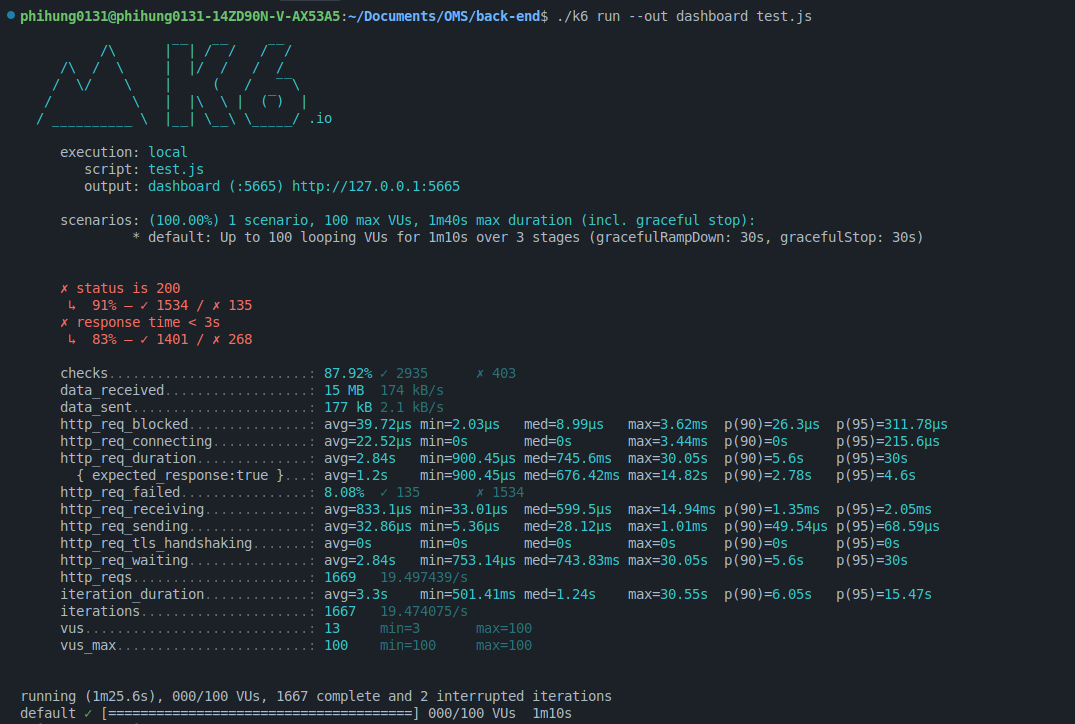
\includegraphics[width=1.0\textwidth]{Images/hienthuc/test_nfr_res.png}
    \vspace{0.5cm}
    \caption{Kết quả kiểm thử}
    \label{fig:k6_result}
\end{figure}

\subsubsection{Phân tích}
\begin{itemize}
    \item \textbf{Checks}: 87.92\% các yêu cầu vượt qua kiểm thử, còn lại 12.08\% thất bại (403 trường hợp). Lý do chính là một số API có tham số chưa chính xác hoặc phản hồi chậm.
    \item \textbf{Thời gian phản hồi trung bình}: 
        \begin{itemize}
            \item Tất cả request: \textbf{2.84s}.
            \item Với các phản hồi hợp lệ (status 200): \textbf{1.2s}, trong đó 95\% các request nằm trong khoảng \textbf{< 4.6s}.
            \item Trung vị (\textit{median}) = 745.6ms, cho thấy đa số request thực tế phản hồi nhanh.
        \end{itemize}
    \item \textbf{Tỉ lệ lỗi}: 8.08\% request thất bại (timeout hoặc lỗi phía server).
    \item \textbf{Thông lượng}: hệ thống xử lý trung bình 19.5 request/giây với 100 người dùng đồng thời.
    \item \textbf{Tài nguyên mạng}: thời gian kết nối (connecting), chờ mở kết nối (blocked), gửi và nhận dữ liệu đều rất nhỏ (micro giây), chứng tỏ nghẽn chủ yếu nằm ở khâu xử lý trên server chứ không phải mạng.
    \item \textbf{Iteration duration}: trung bình 3.3s, với 95\% vòng lặp kết thúc dưới 15.47s. Một số request cá biệt chậm tới 30s, ảnh hưởng đáng kể đến p(95).
\end{itemize}

\subsubsection{Kết luận}
Kết quả kiểm thử cho thấy hệ thống \textbf{cơ bản đáp ứng được yêu cầu phi chức năng}: phần lớn các request hoàn thành dưới 3 giây, phù hợp với tiêu chuẩn phản hồi của hệ thống thời gian thực. Tuy nhiên, vẫn tồn tại khoảng 8\% lỗi và một số request kéo dài tới 30 giây. Do đó, cần tiếp tục tối ưu hiệu năng xử lý ở phía backend (các API phức tạp, thao tác cơ sở dữ liệu) để giảm thiểu các trường hợp chậm trễ này.

\subsection{Tổng quan LightHouse}

Công cụ Google LightHouse được sử dụng để đánh giá hiệu năng, khả năng truy cập, tuân thủ các thực hành tốt nhất và tối ưu hóa SEO cho ứng dụng.  
Các chỉ số được chấm theo thang điểm 100, với bốn hạng mục chính:  

\begin{itemize}
    \item \textbf{Performance}: đo lường tốc độ tải và khả năng phản hồi của trang.  
    \item \textbf{Accessibility}: đánh giá khả năng truy cập cho người dùng, đặc biệt là người khuyết tật.  
    \item \textbf{Best Practices}: kiểm tra các lỗi bảo mật, sử dụng HTTPS, và các khuyến nghị từ Google.  
    \item \textbf{SEO}: đánh giá mức độ thân thiện với công cụ tìm kiếm.  
\end{itemize}

Kết quả kiểm thử được thực hiện trên nhiều màn hình chức năng:

\begin{itemize}
    \item \textbf{Trang chủ (Homepage)}  
    \begin{figure}[H]
        \centering
        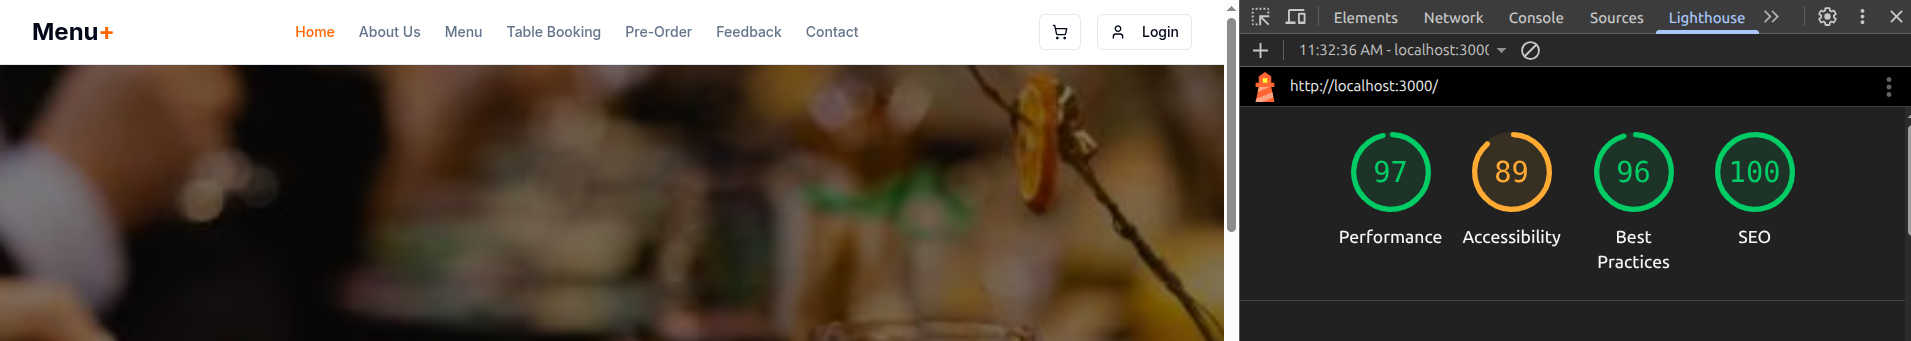
\includegraphics[width=14cm]{Images/hienthuc/lh_homepage.png}
        \vspace{0.5cm}
        \caption{Đánh giá LightHouse Trang chủ (Homepage)}
        \label{fig:lh_homepage}
    \end{figure}
    Điểm số đạt được: Performance 97, Accessibility 89, Best Practices 96, SEO 100.  

    \textit{Nhận xét:} Trang chủ có hiệu năng khá tốt, cần tối ưu thêm Accessibility.  

    \item \textbf{Kitchen Display System (KDS)}  
    \begin{figure}[H]
        \centering
        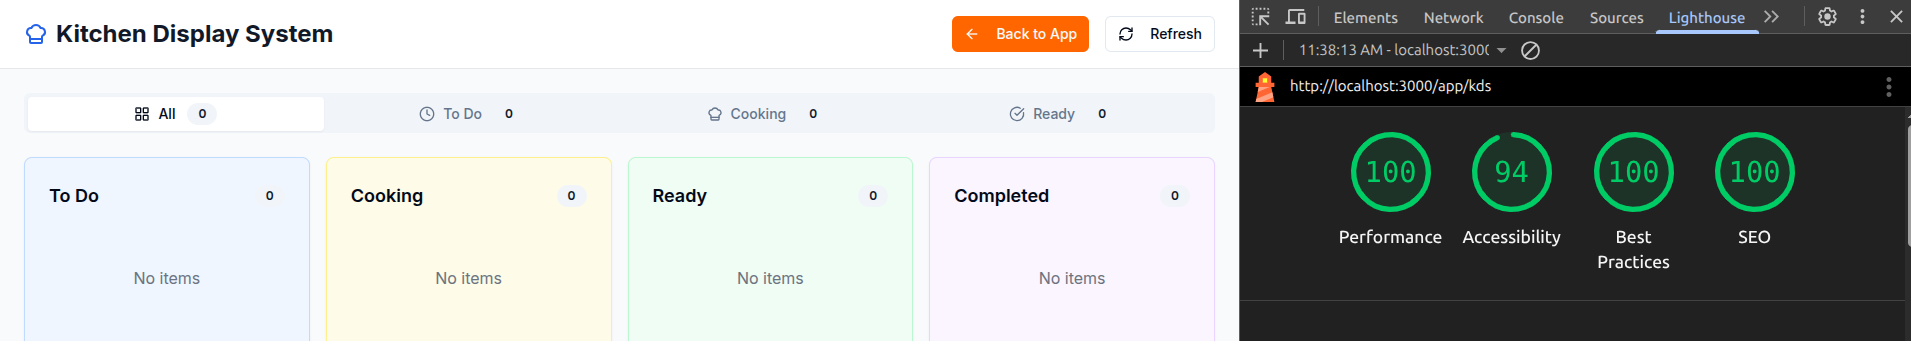
\includegraphics[width=14cm]{Images/hienthuc/lh_kds.png}
        \vspace{0.5cm}
        \caption{Đánh giá LightHouse KDS}
        \label{fig:lh_kds}
    \end{figure}
    Điểm số đạt được: Performance 100, Accessibility 94, Best Practices 100, SEO 100.  

    \textit{Nhận xét:} KDS đạt điểm gần như tuyệt đối, đáp ứng đầy đủ yêu cầu phi chức năng.  

    \item \textbf{Trang Menu}  
    \begin{figure}[H]
        \centering
        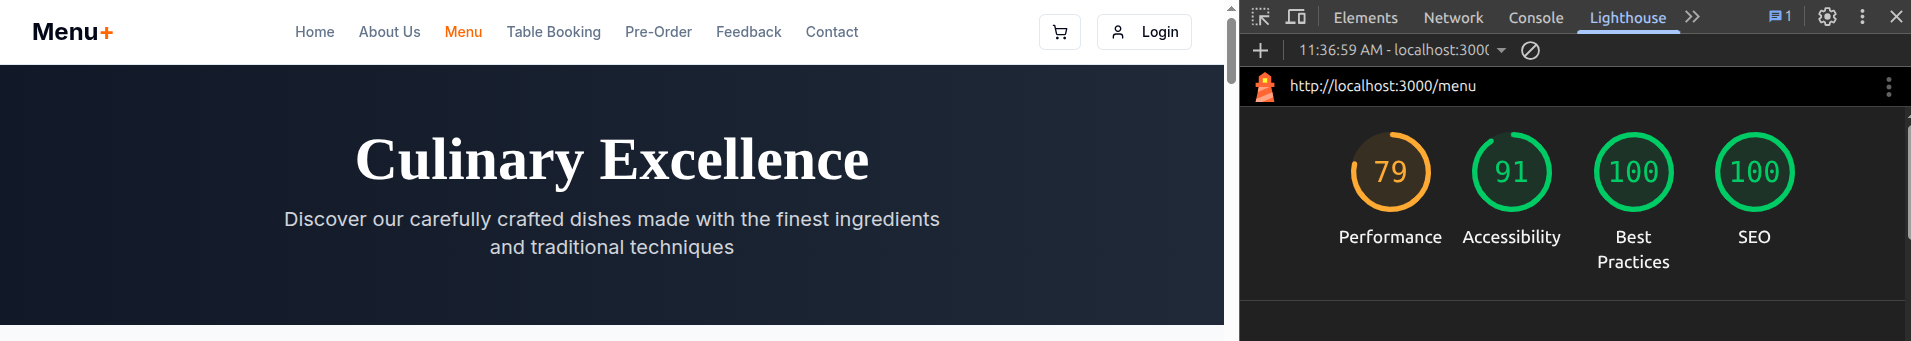
\includegraphics[width=14cm]{Images/hienthuc/lh_menu.png}
        \vspace{0.5cm}
        \caption{Đánh giá LightHouse trang Menu}
        \label{fig:lh_menu}
    \end{figure}
    Điểm số đạt được: Performance 79, Accessibility 91, Best Practices 100, SEO 100.  

    \textit{Nhận xét:} Cần cải thiện hiệu năng (Performance) để đảm bảo trải nghiệm người dùng tốt hơn.  

    \item \textbf{POS - Quản lý bàn}  
    \begin{figure}[H]
        \centering
        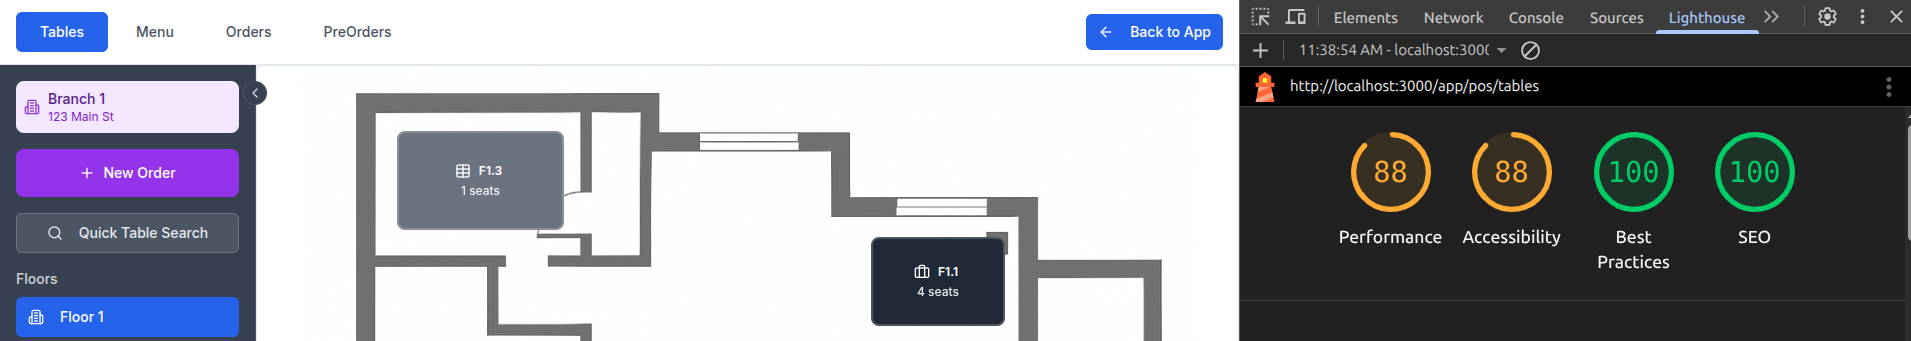
\includegraphics[width=14cm]{Images/hienthuc/lh_pos.png}
        \vspace{0.5cm}
        \caption{Đánh giá LightHouse POS - Quản lý bàn}
        \label{fig:lh_pos}
    \end{figure}
    Điểm số đạt được: Performance 88, Accessibility 88, Best Practices 100, SEO 100.  

    \textit{Nhận xét:} Kết quả khá ổn, nhưng Accessibility vẫn có thể được cải thiện thêm.  

    \item \textbf{Pre-Order}  
    \begin{figure}[H]
        \centering
        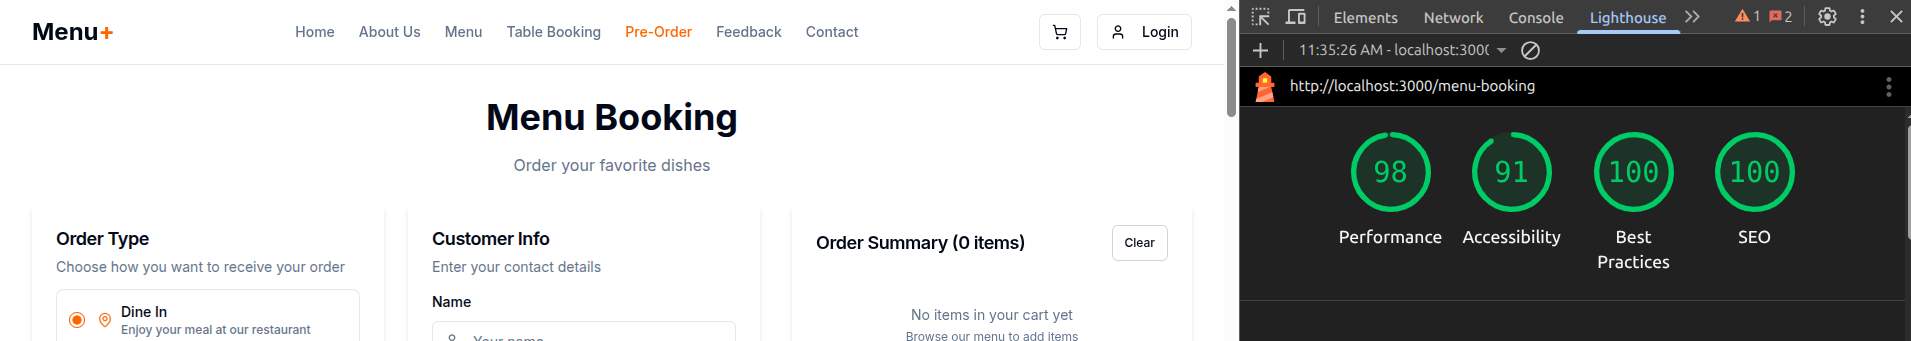
\includegraphics[width=14cm]{Images/hienthuc/lh_preorder.png}
        \vspace{0.5cm}
        \caption{Đánh giá LightHouse Pre-Order}
        \label{fig:lh_preorder}
    \end{figure}
    Điểm số đạt được: Performance 98, Accessibility 91, Best Practices 100, SEO 100.  

    \textit{Nhận xét:} Hiệu năng rất tốt, đảm bảo đáp ứng yêu cầu người dùng.  

    \item \textbf{Table Booking}  
    \begin{figure}[H]
        \centering
        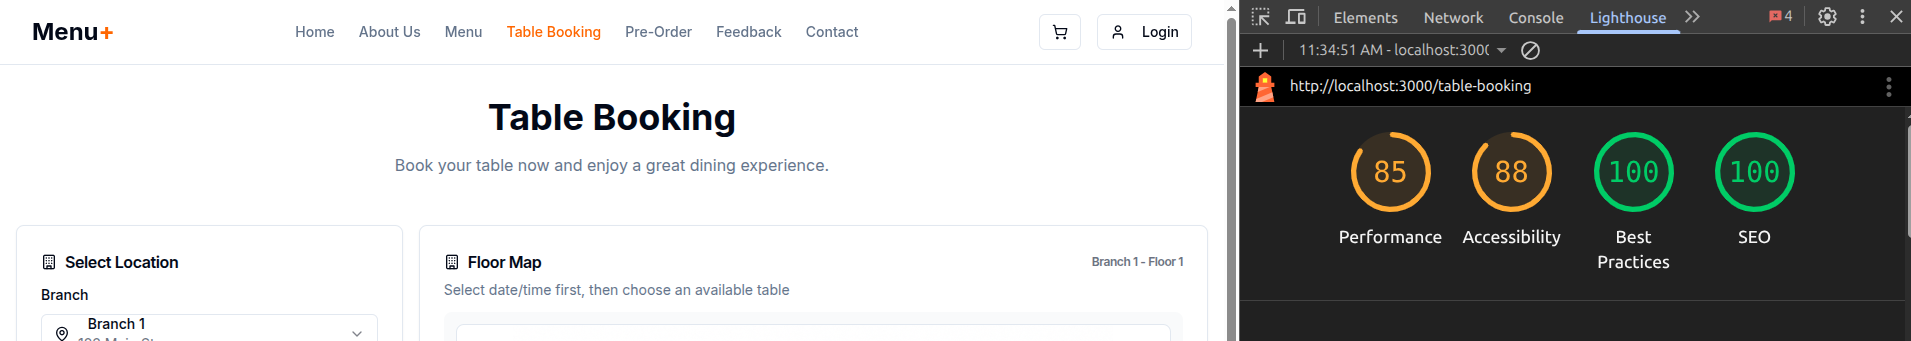
\includegraphics[width=14cm]{Images/hienthuc/lh_tablebooking.png}
        \vspace{0.5cm}
        \caption{Đánh giá LightHouse Table Booking}
        \label{fig:lh_tablebooking}
    \end{figure}
    Điểm số đạt được: Performance 85, Accessibility 88, Best Practices 100, SEO 100.  

    \textit{Nhận xét:} Cần cải thiện hiệu năng và Accessibility, đặc biệt khi hiển thị sơ đồ bàn.  
\end{itemize}

\textbf{Kết luận:}  
Các kết quả trên cho thấy hầu hết các module đều đạt điểm cao về Best Practices và SEO (đều 100), chứng tỏ hệ thống tuân thủ tốt các quy chuẩn kỹ thuật và thân thiện với công cụ tìm kiếm. Tuy nhiên, hiệu năng (Performance) và khả năng truy cập (Accessibility) ở một số trang vẫn còn hạn chế, cần tiếp tục tối ưu về tốc độ tải và khả năng tiếp cận cho mọi đối tượng người dùng.
